\documentclass[12pt,a4paper]{article}
\usepackage[slovene]{babel}
\usepackage{amsmath}
\usepackage{amsfonts}
\usepackage{amssymb}
\usepackage{graphicx}
\usepackage{lmodern}
\usepackage{hyperref}
\usepackage{xcolor}
\usepackage[left=2cm,right=2cm,top=2cm,bottom=2cm]{geometry}
\author{Tina Zwittnig 64200432}
\title{Poročilo 3. vaje pri predmetu OVS \\ interpolacija in decimacija slik}

\begin{document}
\maketitle
\pagebreak
\section{Interpolacijsko območje}
\emph{Določite interpolacijsko sliko kot območje velikosti X × Y = 65 × 50 slikovnih elementov v
dani sliki, pri čemer se prvi slikovni element območja nahaja na lokaciji (x, y) = (75, 30)
slikovnih elementov v dani sliki.\\
Priložite sliko dobljenega interpolacijskega območja. Priložite tudi sliko histograma
interpolacijskega območja ter zapišite minimalno, maksimalno in povprečno sivinsko
vrednost območja.\\}
\begin{figure}[h!]
\centering
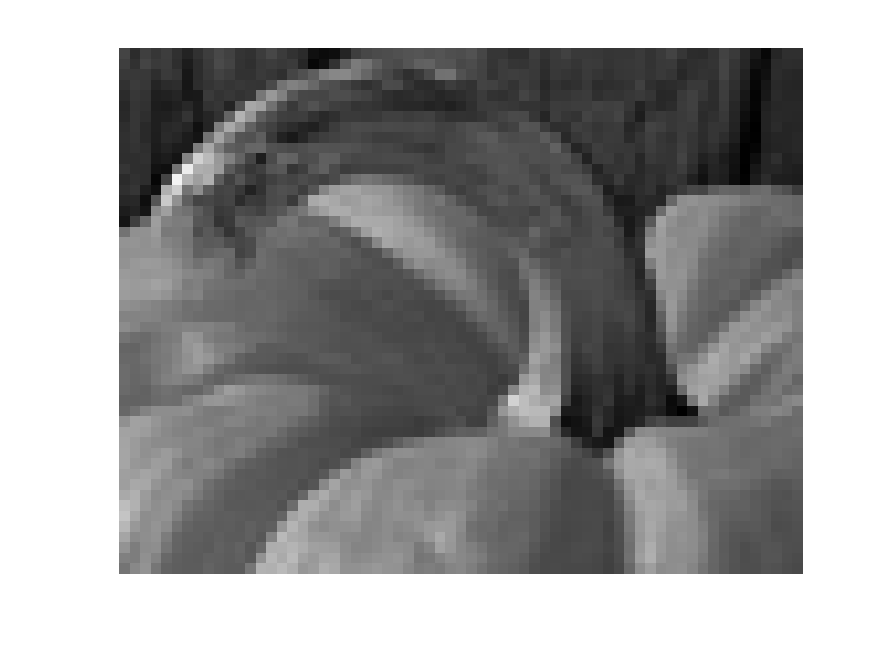
\includegraphics[scale=0.7]{../pictures/prikaz_obmocja.png}
\caption{interpolacijsko območje - originalna slika}
\end{figure}

\begin{figure}[h!]
\centering
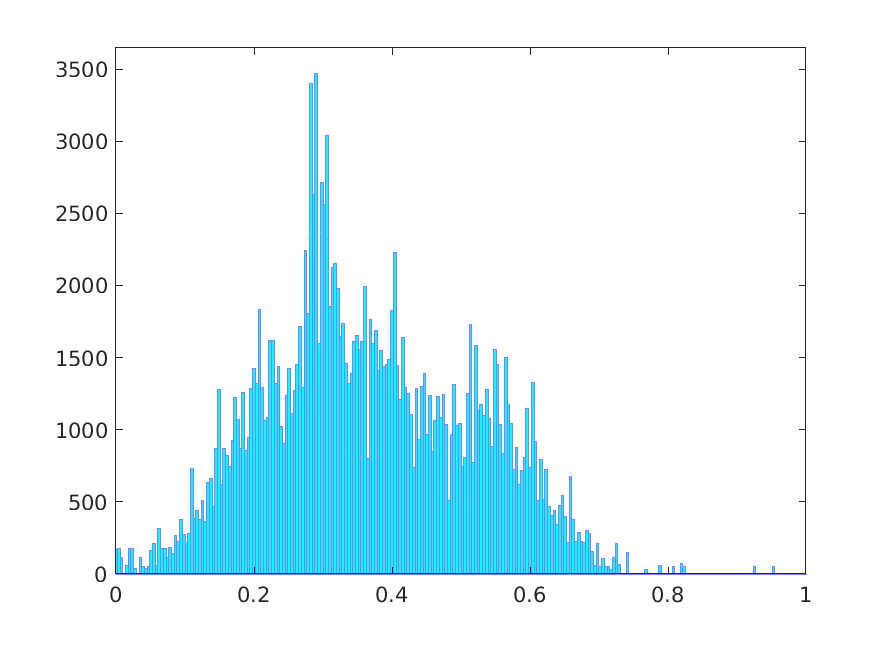
\includegraphics[scale=0.7]{../pictures/histogram_obmocja.png}
\caption{histogram danega območja}
\end{figure}

Maksimalna sivinska vrednost znaša 243, minimalna sivinska vrednost je 0, povprečna sivinska vrednost pa znaša 93.5997.


\section{interpolacija ničtega reda}
\emph{Kaj so prednosti in kaj slabosti interpolacije ničtega reda?\\
Priložite sliko interpoliranega območja velikosti X × Y = 600 × 300 slikovnih elementov,
pridobljenega z interpolacijo ničtega reda interpolacijskega območja. \\
Priložite tudi sliko
histograma interpoliranega območja ter zapišite minimalno, maksimalno in povprečno
sivinsko vrednost interpoliranega območja.\\}

Prednosti interpolacije ničtega reda so, da je računsko enostavna in s tem hitra pri računanju. Slabost pa je, da slika, ki nastane je kockasta in izgubimo nekatere podatke o sliki, ker izberemo najbližjega soseda. Če interpoliramo kakšno sliko, kjer so razlike med sosednimi piksli zelo velike, izgubimo kar nekaj podatkov s tem, da vzamemo najbližjega.  \\

\begin{figure}[h!]
\centering
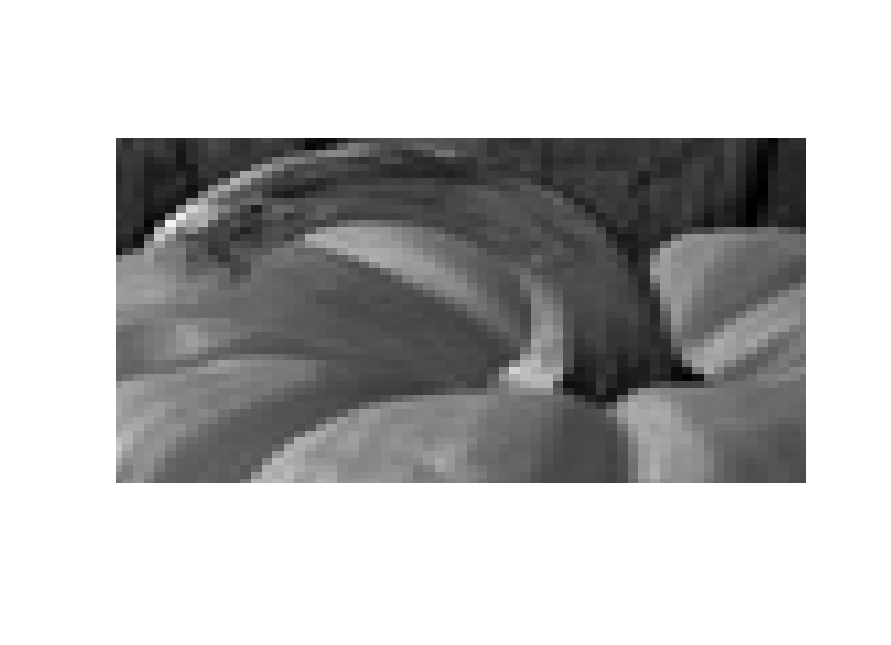
\includegraphics[scale=0.7]{../pictures/prikaz_nictega.png}
\caption{Slika interpolirana z ničtim redom}
\end{figure}
Na sliki je prikazana slika, ki jo dobimo, če dano sliko interpoliramo z ničtim redom v velikosti 600x300. Vidimo lahko slabost interpolacije - kockast prikaz. 
\pagebreak

\begin{figure}[hbtp]
\centering
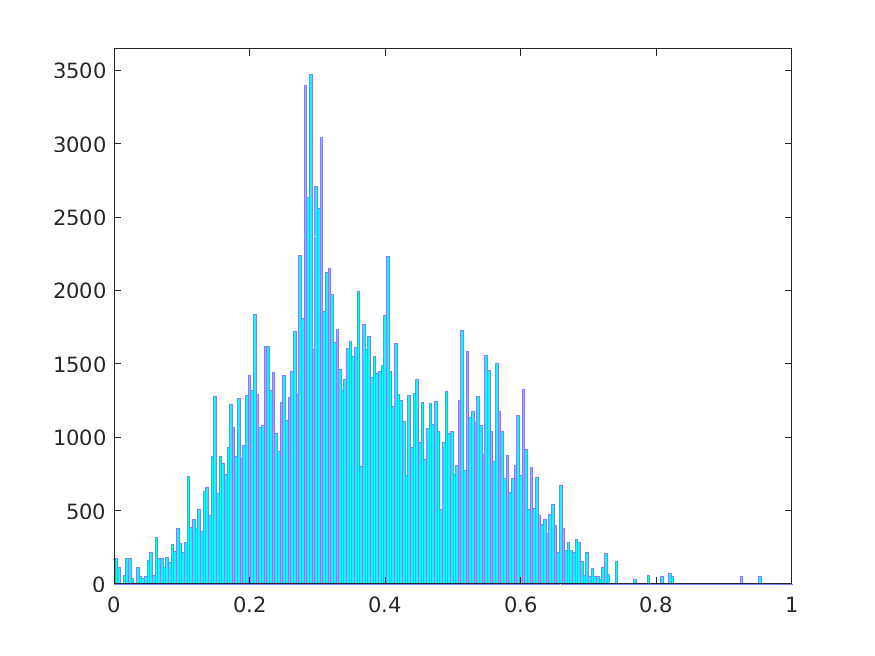
\includegraphics[scale=0.7]{../pictures/histogram_nictega.png}
\caption{pripadajoči histogram interpolirane slike z ničtim redom}
\end{figure}
Maksimalna sivinska vrednost slike z interpolacijo ničega reda je 243, minimalna vrednost je 0, povprečna pa je 93.6990. 

Vrednosti se približno ujemajo z originalno sliko. Prav tako histogram ohrani svojo obliko. 
\section{interpolacija prvega reda}
\emph{Kaj so prednosti in slabosti interpolacije prvega reda?\\
Priložite sliko interpoliranega območja velikosti X × Y = 600 × 300 slikovnih elementov,
pridobljenega z interpolacijo prvega reda interpolacijskega območja. Priložite tudi sliko
histograma interpoliranega območja ter zapišite minimalno, maksimalno in povprečno
sivinsko vrednost interpoliranega območja.}

Prednosti interpolacije prvega reda so, da pri interpoliranju ne vzame vrednosti le najbližjega soseda, ampak uteženo upošteva vrednosti vseh sosednih pikslov. S tem ne izgubimo toliko podatkov o sliki in slika ni tako kockasta ampak se meje pikslov nekoliko zabrišejo. Slabost interpolacije prvega reda je, da je računsko zahtevnejša kot interpolacija ničtega reda, saj mora pogledati vrednosti vseh sosedov in jih nato ustrezno sešteti. Zaradi večjega števila operacij je ta interpolacija počasnejša od interpolacije prvega reda. \\
\pagebreak
\begin{figure}[h!]
\centering
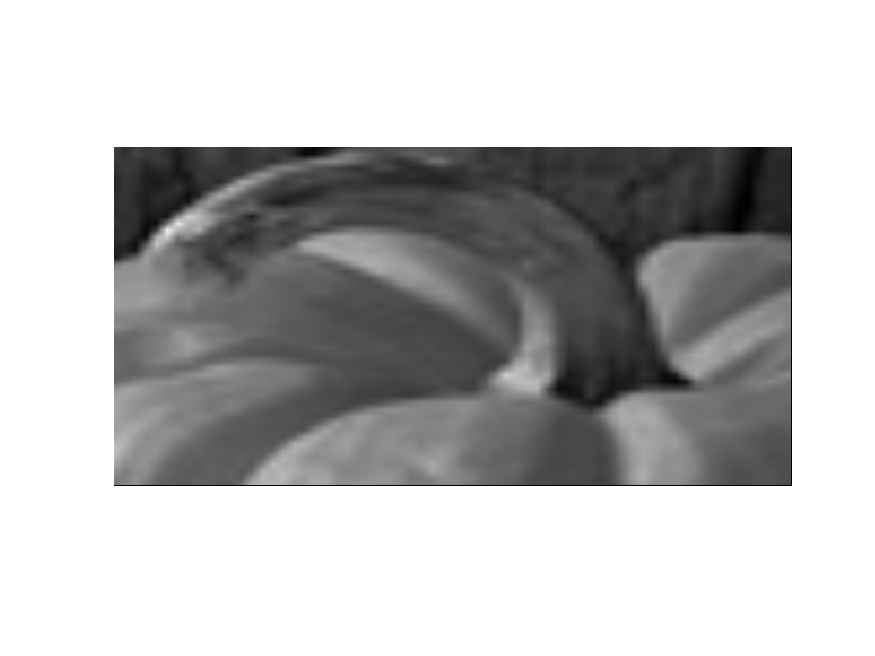
\includegraphics[scale=0.7]{../pictures/prikaz_prvega.png}
\caption{Slika interpolirana z prvim redom}
\end{figure}
\begin{figure}[h!]
\centering
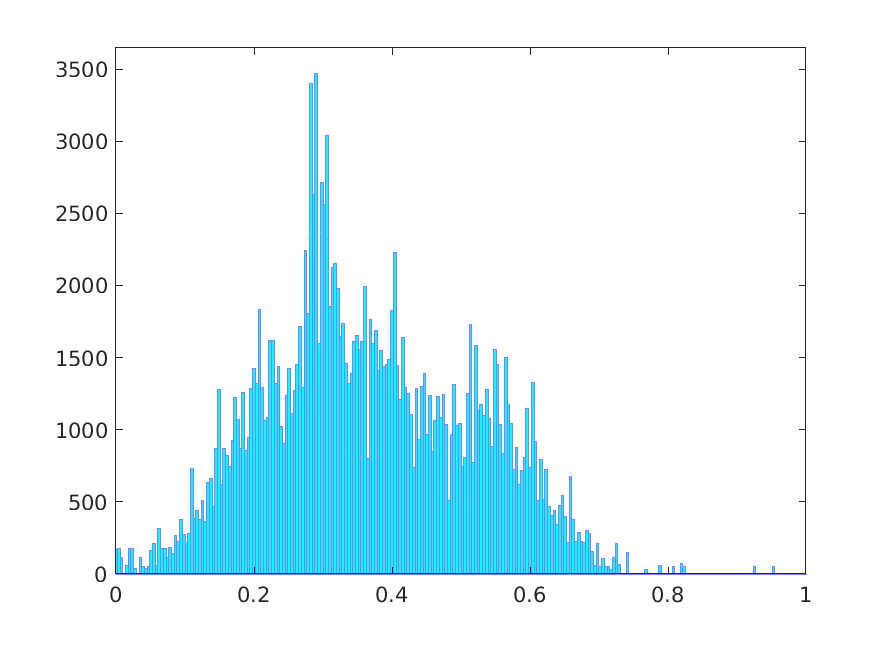
\includegraphics[scale=0.7]{../pictures/histogram_prvega.png}
\caption{Histogram slike interpolirane z prvim redom}
\end{figure}\\
Maksimalna sivinska vrednost slike z interpolacijo prvega reda je 237, minimalna vrednost je 0, povprečna vrednost pa je 92.6631. Vrednosti se nekoliko razlikujejo od originalne slike, vendar so dovolj blizu. Histogram podobno kot interpolacija ničtega reda ohranja svojo obliko.
\section{interpolacije višjih redov} 
\emph{Kaj dosežemo z interpolacijami višjih redov, npr. z interpolacijo tretjega reda?\\}

Z interpolacijami višjih redov dosežemo vedno mehkejše prehode in s trem vedno manj kockastih prikazov. Pri interpolaciji ne upoštevamo le sosedov ampak širše območje okoli dane lokacije. S tem so prehodi bolj zvezni in lahko sliko boljše ločljivosti prikažemo na zaslonu manjše ločljivosti, brez da bi prišlo do prevelikih popačenj. 
\section{Prikazovanje slik z interpolacijo drugačne dimenzije}
\emph{Pri prikazovanju slik vzpostavite dimenzijsko sorazmerje med interpolacijskim in inter-
poliranim območjem (tj. območji morata biti enakih fizičnih dimenzij), in sicer tako, da
spremenite obstoječo funkcijo displayImage z dodatnima vhodnima argumentoma iGridX
in iGridY} :\\
\begin{center}
\texttt{\textcolor{blue}{function} displayImage(iImage, iTitle, iGridX, iGridY)},
\end{center}
\emph{ki predstavljata vektorja položajev slikovnih elementov v x in y smeri ter
neposredno ustrezata argumentoma x in y Matlabove funkcije} \texttt{image(x,y,C)}\\
(\url{https://www.mathworks.com/help/matlab/ref/image.html} ).\\
\emph{Priložite sliki interpoliranih območij, pridobljenih z interpolacijo ničtega oz. prvega reda
interpolacijskega območja, ki sta v dimenzijskem sorazmerju z interpolacijskim območjem.\\
Priložite tudi programsko kodo spremenjene funkcije} \texttt{displayImage}.\\

Koda funkcije \texttt{displayImage} z dodanimi vhodnimi parametri.
\begin{verbatim}
function graph = displayImage(iImage, iTitle, iGridX, iGridY)
% prikaže sliko na zaslonu.
% vhodni elementi: 
%   iImage - matrika, ki predstvlja sliko
%   iTitle - naslov slike
%   iGridX - čez katere x vrednosti naj bo prikazana slika 
%       podan v vektorju [x1 x2] 
%   iGridY - čez katere y vrednosti naj bo prikazana slika
%       podan v vektorju [y1 y2]
% izhodni podatki:
%   graph - objekt tipa figure, ki predstavlja prikazoano sliko

slika = figure('Name', iTitle, 'Color', [1 1 1]);
% določi barvno lestvico
cmap = linspace(0,1, 256)';
cmap = [cmap cmap cmap];
colormap(cmap);
graph = image(iGridX, iGridY, uint8(iImage));
axis image;
axis off;
end
\end{verbatim}

\pagebreak

\begin{figure}[hbtp]
\centering
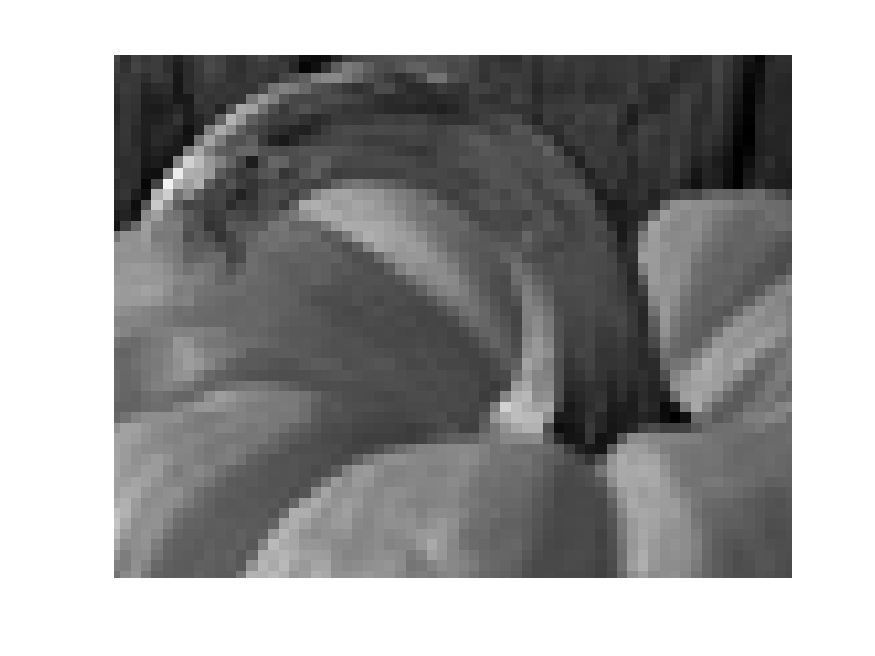
\includegraphics[scale=0.7]{../pictures/popravljen_prikaz_nictega.png}
\caption{Popravljen prikaz slike z interpolacijo ničtega reda}
\end{figure}

\begin{figure}[hbtp]
\centering
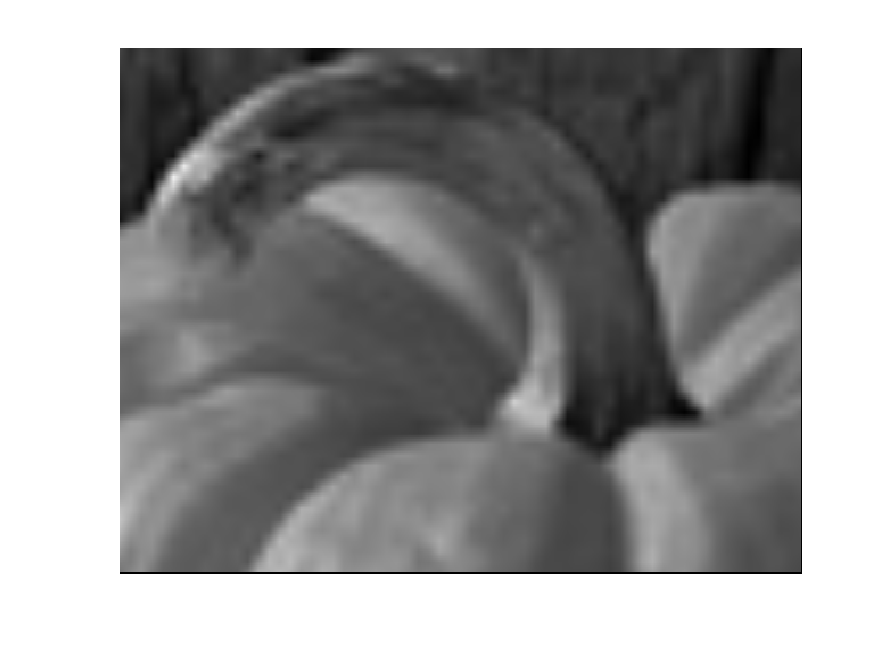
\includegraphics[scale=0.7]{../pictures/popravljen_prikaz_prvega.png}
\caption{Popravljen prikaz slike z interpolacijo prvega reda}
\end{figure}
Slike pri popravljenem prikazu so v istih fizičnih dimenzij kot originalna slika. 



\end{document}
